\documentclass[A4]{scrartcl}
\usepackage[paper=a4paper,left=10mm,right=10mm,top=25mm,bottom=25mm]{geometry}
\usepackage[utf8]{inputenc}
\usepackage{graphicx}

\begin{document}
  \addsec{Verständnisfragen}
  Welche zwei Parameter bestimmen die Bandbreite einer rückgekoppelten\\ 
  Operationsverstärkerschaltung?\\
  \\
  Antwort: Bandbreite des OP (Transitfrequenz) $F_t$ + Verstärkung der Rückkopplung ($A_0$)\\\\
  Welche zwei Eigenschaften sind für einen VC-operationsverstärker charakteristisch?\\
  \\
  Antwort: Eingangswiderstand ist sehr groß (Spannungseingang), Ausgangswiderstand ist sehr groß(Stromausgang)\\\\
  Im Handel sind verschiedene Arten von Operationsverstärkern verfügbar. Diese werden durch zwei Buchstaben beschrieben: XY-Operationsverstärker. Was wird durch die Buchstaben beschreiben und welche Optionen sind verfügbar?\\
  \\
  Antwort: X = Eingang, Y = Ausgang\\
  V = Spannungs-Ein/Ausgang, C= Strom-Ein/Ausgang.\\
  Verfügbar sind: VV,VC,CV,CC - Operationsverstärker \\\\
  Worauf müssen sie bei der Verwendung eines VC-Operationsverstärkers achten ? Erklären sie am Beispiel eines Spannungsfolgers.\\
  \\
  Antwort: Bei der Rückführung muss der Ausgangsstrom in eine Spannung konvertiert werden (z.B. über einen Widerstand), deshalb ist eine direkte Verbindung von Ausgang und Eingang nicht Möglich.\\\\
  Was bzw. welches Bauteil definiert die Eingangsimpedanz einer nicht-invertierenden Verstärkerschaltung?\\
  \\
  Antwort:Der Eingangswiderstand des OP's\\\\
  Was versteht man unter der common mode rejection ratio CMRR?\\
  \\
  Antwort: Die Fähigkeit eines realen Operationsverstärkers seinen Ausgang bei Symmetrischen Eingangssignalen möglichst wenig zu ändern.\\
  (Symmetrische Änderungen des Eingangs haben aufgrund von Assymetrien/Nichtidealitäten an den Eingängen eine Änderung am Ausgang zur Folge)\\
  Sie ist damit ein Maß für den Einfluss der Eingangsspannung auf die Ausgangsspannung\\
  CMRR = Common Mode Rejection Ratio\\\\
  Was versteht man unter power supply rejection Ratio PSRR?\\
  \\
  Antwort: Die PSRR gibt ein Maß für den Einfluss der Versorgungsspannung auf den Ausgang an.\\\\
  Erläutern Sie die Unterschiede zwischen einem normalen Operationsverstärker, einem single Supply und einem rail-to-rail OP? (Eventuell fertigen Sie zur Erklärung eine kleine Skizze an).\\
  \\
  Antwort: 
  normaler OPV (Symmetrische Versorgung): Versorgung mit $+U_V$, $-U_V$, Nutzbereich $\approx [(-U_V +1/2V); (+U_V -1/2)V]$\\
  single Supply OPV (Asymmetrische Versorgung): Versorung mit $+U_V$, Nutzbereich $\approx [(0V+ "x"mV); (Uv -1/2V)]$ \\
  Rail to Rail OPV (Symmetrische Versorgung): Versorung mit $+U_V$, $-U_V$, Nutzbereich $\approx [(-U_V + "x"mV); (+U_V - "x"mV)]$\\\\
  Nennen sie zwei OP-Grundschaltungen, die häufig für die Realisierung von Filtern höherer Ordnung verwendet werden.\\
  \\
  Antwort: Sallen - Key Filter, Multiple Feedback Filter, Universal/State-Variable-Filter\\\\
  Warum können Sie einen Operationsverstärker als Komparator einsetzen, einen Komparator aber nicht als Operationsverstärker?\\
  \\
  Antwort: Der Ausgang des Komparator kann meist nur $+U_s$ und $-U_s$\\\\
  Was sind die charakteristischen Eigenschaften eines Instrumentenverstärkers?
  \\
  Antwort: sehr hoher Eingangswiderstand, dadurch wenig Beeinflussung der Messung durch Nichtidealitäten.\\\\
  Wann wird er verwendet?\\
  \\
  Antwort: Präzise Messschaltungen und Messung\\ von Schaltungen mit hohen Ausgangswiderständen.\\\\
  Skizzieren sie das Blockschaltbild für einen (Einquadranten-)Analogmultiplizierer? Aus welchen Grundelementen wird dieser typischerweise aufgebaut?\\
  \\
  Antwort:\\\\
  Wozu dient die Frequenzgankompensation in einem Operationsverstärker? Nennen sie zwei typische Implementierungen.\\
  Antwort:
  \\
  Erklären sie, warum bei einem vereinfachten Dreiecksgenerator nicht immer ein Dreieck am Ausgang entsteht? Von welchen Bauteilen ist dies abhängig(Skizze)?\\
  \\
  Antwort:
  Was bzw. welches Bauteil definiert die Eingangsimpedanz einer invertierenden Verstärkerschaltung?\\
  \\
  Antwort:
  Was bzw. welchess Bauteil definiert die Eingangsimpedanz einer Integratorschaltung?\\
  \\
  Antwort: Der Widerstand vor dem Kondensator.\\\\
  Warum setzt man in der Praxis eine reine Integratorschaltung nur selten ein? Unter welchen Bedingungen /in welchen Schaltungen wird sie dennoch verwendet? Warum ist die Verwendung dort möglich?\\
  \\
  Antwort: Die reine Integratorschaltung stellt einen Tiefpass dar und ist nur bei Frequenzen $F >> f_C$ ein Integrierer(Linearität der E-Fkt der Ladekurve)\\
  Da die Nichtidealitäten (Offset- und Basisströme) mit integriert werden, neigt der Integrierer dazu sich über die Laufzeit auf einer der Versorgungsspannungen festzulegen.\\
  Ein Integrierer ist bei niedrigen Frequenzen deshalb nur mit einem Parallelwiderstand oder einer automatischen Entladeschaltung nutzbar.\\\\
  Nennen sie zwei Optionen um das Weglaufen der Ausgangsspannung in einer Integratorschaltung zu verhindern? Wann verwenden sie welche Option ?\\
  \\
  Antwort: Entladewiderstand parallel zum Kondensator , Entladeschaltung (vgl. Öffner)\\\\
  Nennen Sie drei in der Vorlestung diskutierte Filtercharakteristiken.
  \\
  Antwort: Bessel, Butterworth, Tschebyscheff, Kritische Verstärkung, Cauer-Filter.\\\\
  Erläutern sie den Unterschied zwischen der Eigenfrequenz $f_0$ und der Grenzfrequenz $f_c$ eines Tiefpasses 2. Ordnung.\\
  \\
  Antwort:
  $f_c = $ Frequenz bei der der Ausgang Verstärkung-3DB beträgt (Bsp: $A_0 = 10dB - 3dB = 7dB $)\\
  $f_0 = $ Frequenz bei der$\varphi(f_0) = -90^\circ$\\\\
  Ein state-variable-Filter wird häufig als Universal-Filter bezeichnet. Erklären Sie warum?\\
  \\
  Antwort: 1. man kann mit einem State Variable Filter alle Filtertypen (gleichzeitig) realisieren (Hochpass, Tiefpass, Bandpass, Bandsperre).\\\\
  Sie möchten einen invertierenden Verstärker bauen. in Ihrer Bastelkiste finden sie aber nur einen LM339 Komparator IC. Was machen sie? Warum?\\
  \\
  Antwort: IC ist nicht nutzbar, da Ausgang nur Totem-Pole-Endstufe($ +U_S$, $-U_S$)\\
  Keine Zwischenwerte möglich\\
  Daher: neue IC's bestellen (man kann einene Komparator nicht als OPV nutzen)\\\\
  Warum werden die Eigenschaften der meisten Operationsverstärkerschaltungen nicht durch die Eigenschaften des Operationsverstärkers, sondern im Wesentlichen durch die externen Komponenten bestimmt ?\\
  \\
  Antwort: $\frac{U_out}{U_in} = \frac{G}{1-G\cdot H} = -\frac{1}{H}$ für $G\cdot H >> 1$\\\\
  Sie haben im Labor eine ideale Differenzierer-Schaltung aufgebaut.\\
  Zum Testen der Schaltung verwenden sie ein Dreieckssignal.\\
  Leider hat das Ausgangssignal keinen rechteckförmigen Verlauf, sondern seltsame "Zacken" an den Flanken.\\
  Sie haben festgestellt das die "Zacken" mittels eines Widerstands in Reihe zum Kondensator entfernen können.\\
  Erklären sie wodurch die "Zacken" entstehen und warum sie mit dem Widerstand entfernt werden können. Eventuell hilft eine Zeichnung weiter.\\
  \\
  Antwort: Der Operationsverstärker wird durch den Kondensator kapazitiv belastet.\\
  Dies verursacht Stabilitätsprobleme (System 2. Ordnung) der Kondensatorladestrom wird durch den Widerstand begrenzt. 
  Was versteht man unter der Phasenreserve eines rückgekoppelten Systems?\\
  \\
  Antwort: Phasenreserve $ \varphi_r = 180^\circ - \varphi$\\
  Bei einer Verstärkung von $|A|=0dB=1$\\
  Maß für die Stabilitätsreserven eines Systems\\\\
  Erklären sie Stichpunktartig den Unterschied zwischen Differenzverstärker und einem Differenzierer?\\
  \\
  Antwort:
  Differenzverstärker: Verstärkt die Differenz zwischen invertierenden und nicht invertierenden Eingang (Math. Operation der Subtraktion)\\
  Differenzierer: Führt die Operation der Differentiation auf ein Eingangsfunktional aus.\\\\
  Warum können Sie in einem Rechteck-Dreieck Generator einen idealen integrator einsetzen und benötigen keinen Tiefpass?\\
  \\
  Antwort: Der Integrator wird kontinuierlich Ge-und Entladen, er wird deswegen in einer Art Rückkopplung betrieben.\\\\
  Nennen Sie drei Filtertypen, die häufig für die Auslegung von Filtern höherer Ordnung verwendet werden.\\
  \\
  Antwort: Bessel, Butterworth, Tschebyscheff, Kritische Dämpfung\\\\
  \addsec {OPV-Schaltungen}
  Gegeben sei folgende Schaltung:\\
  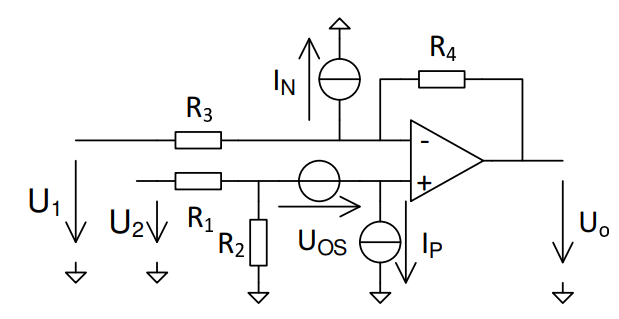
\includegraphics{Schaltung1.png}\\
  a) Bestimmen Sie die Ausgangsspannung $U_{out}$ als Funktion der gegebenen Größen.\\
  $U_{out} = f(U_1,U_2,U_{os},I_N,I_P)$\\
  b) Vereinfachen sie den Ausdruck für $R_1 = R_3, R_2 = R_4$ und $I_N = I_B + 0.5 I_{OS}, I_P = I_B-0,5I_{OS}$\\\\
  Die Aussteuergrenzen sollen mit $\pm 15V$ angenommen werden.\\
  a) Schreiben sie jweiels die Potentiale bzw. Ströme in die Kästchen:\\
  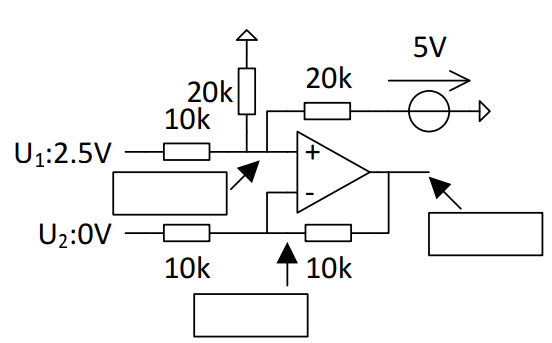
\includegraphics{Schaltung2.png}\\\\
  b) Schreiben sie jweiels die Potentiale bzw. Ströme in die Kästchen:\\
  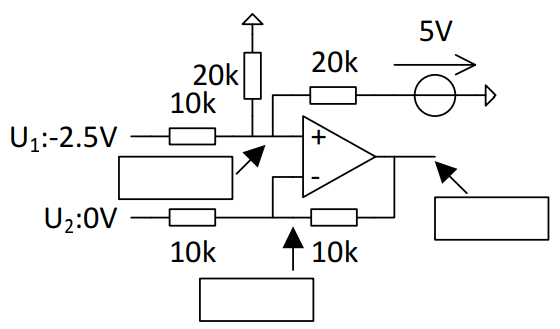
\includegraphics{Schaltung3.png}\\\\
  
\end{document}
